% AKULIN R2 CP07 -- figure 6.7, source-traced vector reconstruction.
% Geometry is in pixel-landmark coordinates of the author's reproduced figure.
% Caution: printed curves are NOT measured raw data; no fitted linewidths are asserted.
% Four independent contours: t=0 (foreground) and 100, 200, 300 microseconds.
% Curves use individually identified shoulders/peaks/decays, not template peak functions.
\documentclass[border=6pt]{standalone}
\usepackage{fontspec,unicode-math}
\setmainfont{Noto Serif}
\setmathfont{STIXTwoMath-Regular.otf}
\usepackage{tikz}
\usetikzlibrary{arrows.meta,calc}
\tikzset{
  axis/.style={draw=black,line width=.67pt,-{Latex[length=2.0mm,width=1.25mm]}},
  contour/.style={draw=black,line width=1.05pt,line cap=round,line join=round},
  baseline/.style={draw=black,line width=.65pt,line cap=round},
  tick/.style={draw=black,line width=.57pt},
  lab/.style={font=\fontsize{11.5}{13.8}\selectfont,inner sep=1.1pt},
  smalllab/.style={font=\fontsize{10.5}{12.3}\selectfont,inner sep=1pt}
}
\begin{document}
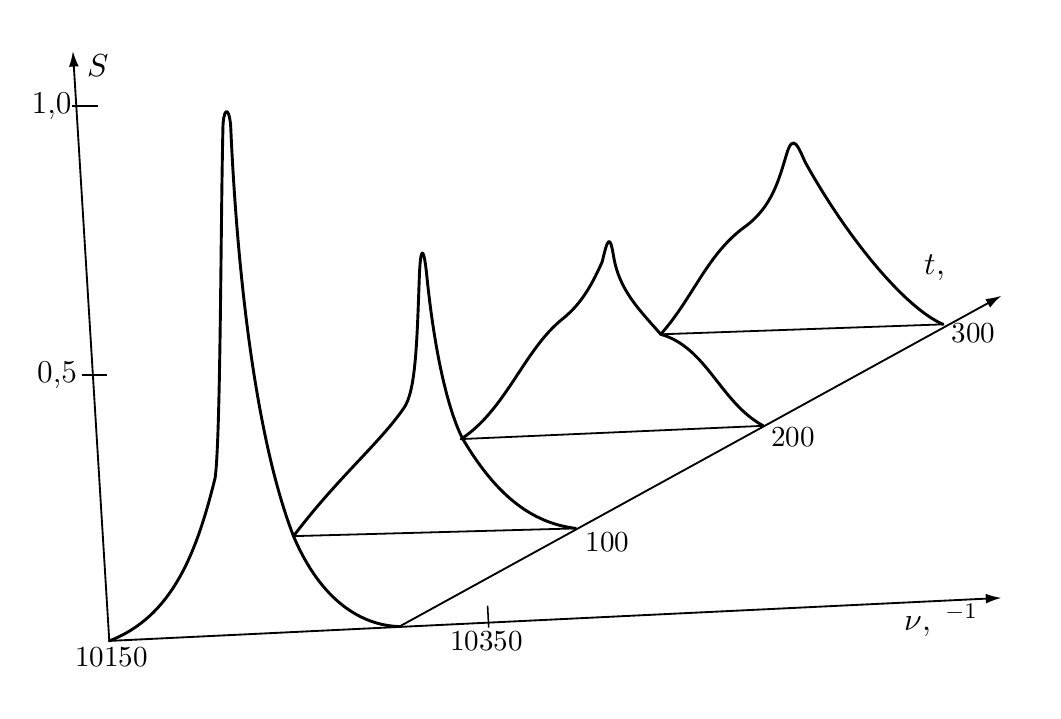
\begin{tikzpicture}[x=.014cm,y=-.014cm]
\path[use as bounding box] (4,-2) rectangle (915,599);
% Original's coordinate geometry is gently skewed by book reproduction;
% plotted coordinates retain that skew instead of silently shifting peaks.
\coordinate (O) at (78,554);
\coordinate (T0) at (341,541);
\coordinate (T100) at (501,452);
\coordinate (T200) at (671,360);
\coordinate (T300) at (834,267);
% Rear contours first: independently traced characteristic shoulders and decay.
\draw[baseline] (578,276)--(834,267);
\draw[contour] (578,276)
 .. controls (608,242) and (620,203) .. (655,178)
 .. controls (679,160) and (685,136) .. (692,113)
 .. controls (698,92) and (703,107) .. (709,120)
 .. controls (746,187) and (799,252) .. (834,267);
\draw[baseline] (397,371)--(671,359);
\draw[contour] (397,371)
 .. controls (438,344) and (454,290) .. (489,262)
 .. controls (504,250) and (514,235) .. (525,210)
 .. controls (530,188) and (532,186) .. (535,204)
 .. controls (540,236) and (558,253) .. (578,276)
 .. controls (620,288) and (632,338) .. (671,359);
\draw[baseline] (245,459)--(501,452);
\draw[contour] (245,459)
 .. controls (286,405) and (322,376) .. (345,343)
 .. controls (356,328) and (357,281) .. (359,227)
 .. controls (360,195) and (363,194) .. (366,224)
 .. controls (373,293) and (385,344) .. (398,370)
 .. controls (428,421) and (460,447) .. (501,452);
% Foreground contour has a narrow almost-vertical peak and asymmetric decay.
\draw[contour] (78,554)
 .. controls (135,532) and (157,475) .. (174,406)
 .. controls (179,368) and (179,173) .. (181,91)
 .. controls (181,72) and (186,67) .. (188,86)
 .. controls (194,223) and (211,371) .. (245,459)
 .. controls (270,518) and (307,540) .. (341,541);
% Physical axes and the oblique time axis are drawn after all contours.
\draw[axis] (78,554)--(887,515);
\draw[axis] (78,554)--(45,19);
\draw[axis] (T0)--(887,241);
\draw[tick] (53,313)--(76,313);
\draw[tick] (44,69)--(68,69);
\node[lab,anchor=east] at (47,69) {1,0};
\node[lab,anchor=east] at (52,313) {0,5};
\node[lab,anchor=west] at (55,32) {$S$};
\draw[tick] (421,522)--(422,542);
\node[smalllab,anchor=north] at (80,557) {$10150$};
\node[smalllab,anchor=north] at (420,542) {$10350$};
\node[lab,anchor=west] at (796,535) {$\nu,\ \mathrm{см}^{-1}$};
\node[smalllab,anchor=north west] at (507,452) {$100$};
\node[smalllab,anchor=north west] at (675,357) {$200$};
\node[smalllab,anchor=north west] at (839,263) {$300$};
\node[lab,anchor=south west] at (814,231) {$t,\ \mathrm{мкс}$};
\end{tikzpicture}
\end{document}
